%% ============================================================================
%% The Exact Error Exponent of Rate-Constrained Decentralized Detection
%% over Time-Varying Networks
%% Target: IEEE Transactions on Information Theory (IEEEtran journal class).
%% Reconstructed manuscript. Author names and affiliations intentionally blank.
%% ============================================================================
\documentclass[journal]{IEEEtran}

\usepackage{amsmath,amssymb,amsfonts}
\usepackage{amsthm}
\usepackage{graphicx}
\usepackage{booktabs}
\usepackage{array}
\usepackage{tikz}
\usepackage{pgfplots}
\pgfplotsset{compat=1.18}
\usetikzlibrary{arrows.meta,positioning,calc,decorations.pathmorphing,backgrounds}
\usepackage[hidelinks]{hyperref}
\usepackage{cite}
\usepackage{xcolor}

\graphicspath{{../Figures/}}

\newtheorem{theorem}{Theorem}
\newtheorem{lemma}{Lemma}
\newtheorem{proposition}{Proposition}
\newtheorem{corollary}{Corollary}
\theoremstyle{definition}
\newtheorem{definition}{Definition}
\theoremstyle{remark}
\newtheorem{remark}{Remark}

\newcommand{\Ecen}{E^{\mathrm{cen}}}
\newcommand{\tib}{\theta_{\mathrm{IB}}}
\newcommand{\tibi}{\theta_{\mathrm{IB},i}}
\newcommand{\tsha}{\theta_{\mathrm{SHA}}}
\newcommand{\Gk}{\Gamma_k}
\newcommand{\Cdib}{C_{\mathrm{DIB}}}
\newcommand{\KL}[2]{D\!\left(#1\,\Vert\,#2\right)}
\newcommand{\R}{\mathbb{R}}
\newcommand{\E}{\mathbb{E}}
\newcommand{\N}{\mathbb{N}}
\DeclareMathOperator{\Var}{Var}

\begin{document}

\title{The Exact Error Exponent of Rate-Constrained\\ Decentralized Detection over Time-Varying Networks}

\author{\thanks{Manuscript submitted for review to the IEEE Transactions on Information Theory.}}

\markboth{IEEE Transactions on Information Theory}%
{Rate-Constrained Decentralized Detection over Time-Varying Networks}

\maketitle

\begin{abstract}
A group of agents each observe a small piece of one phenomenon and must reach the same decision about it, yet
the links between them carry only a few nats per use and the connectivity keeps changing. We determine the exact
best Type-II error exponent that any single agent can achieve for a test against independence when there is no
fusion center. The exponent equals the smaller of two quantities, namely the centralized Stein exponent that
unlimited communication would allow and the information-bottleneck relevance at the long-run minimum cut that
separates the agent from the observations. We prove a converse showing that no fusion-free rate-constrained scheme
can pass this value, and we prove a matching achievability by carrying information-bottleneck descriptions across
the graph with random linear network coding. The two bounds coincide, so the exponent is settled with no gap over
directed graphs that may contain cycles and may change with time. A closed-form Gaussian model turns the result
into a water-filling rule for sharing a budget among unequal agents. An exact optimal-detector measurement, a
genuinely routed network, and an actual finite-field code confirm every prediction to within a few thousandths of
a nat, and show across ten graph families that the achievable exponent depends on the wiring only through this
cut.
\end{abstract}

\begin{IEEEkeywords}
Decentralized detection, error exponents, hypothesis testing, information bottleneck, rate constraints, min-cut,
random linear network coding, time-varying networks, distributed inference.
\end{IEEEkeywords}

%% ===========================================================================
\section{Introduction}\label{sec:intro}
%% ===========================================================================
\IEEEPARstart{I}{magine} a swarm of small drones spread over a wide area after a flood. Each drone sees only the
patch of ground beneath it, so no single drone can answer the one question the rescue team cares about, which is
whether a dam upstream has failed. Any one drone has weak and noisy evidence, yet the drones together, if they
could pool everything they see, could be almost certain. Three facts stop them from simply pooling. The radios
are tiny, so a drone can send only a handful of bits per second and cannot transmit its full camera image. There
is no control tower that gathers all the data and decides, so each drone must reach its own conclusion from what
trickles across the network. The wiring keeps changing, because drones move and links drop and reappear. The
scientific question is how good the collective decision can possibly be under these three constraints, and what
physical quantity sets the ultimate limit.

The right way to grade such a system is not its raw error probability, which depends on how long it runs, but the
speed at which that error falls. When an agent collects more independent samples over time, the probability of a
wrong decision typically shrinks like $e^{-nE}$ in the number of samples $n$, and the constant $E$ is the error
exponent. A large exponent means the error vanishes quickly, a small one means it vanishes slowly, and a zero
exponent means the agent never becomes sure. The exponent is the intrinsic, sample-count
independent grade of a detector, and it is the quantity about which a fundamental limit can be stated. This paper
characterizes the best error exponent that a single agent can reach.

This problem matters well beyond the drone story. Sensor fields watch for intrusions, leaks, or seismic events
with cheap radios and no central server. Fleets of autonomous vehicles must agree on a shared world state over
links that come and go. Edge and datacenter services each hold a slice of telemetry and must decide a global
condition over congested paths. In all of these the same three obstacles appear together, and an engineer who
knows the exponent knows exactly how much link budget is needed to reach a target decision quality, and knows
when buying more bandwidth is wasted because the statistical ceiling has been reached.

The classical theory answers the question only when the obstacles are removed one at a time. When a single
observer feeds a single detector with no rate limit, Stein's lemma fixes the best Type-II exponent at the
Kullback-Leibler divergence between the two hypotheses \cite{chernoff1952,coverthomas2006}. When one rate-limited
link separates an observer from a detector, Ahlswede and Csisz\'ar found the exact exponent for a test against
independence, and it is an information-bottleneck functional of the available rate \cite{ahlswedecsiszar1986}.
When the topology varies over time but the messages carry full belief vectors with no rate limit, the
non-Bayesian social-learning line gives geometric rates of belief concentration governed by a network-averaged
divergence \cite{nou2017,lalitha2018,shahrampour2016}. Each of these results switches off exactly the ingredient
that makes the others hard.

The gap that remains is the intersection that none of them treats, namely a topology that changes with time, the
absence of any fusion center, and a hard Shannon budget on every edge, all present at once. When the three hold
together the problem changes in character. The rate available to an agent is no longer a fixed number but a
random, time-averaged cut of a changing graph. The exponent becomes different at different agents. The
compression and the agreement can no longer be separated, because the very messages that build agreement must
themselves squeeze through the links that are being rate-limited. No prior work characterizes the exponent in
this regime.

Our key insight is that the problem cleanly splits into a network part and a statistics part that never speak to
each other, and that their answers combine by a simple minimum. The network can deliver only so much information
about the hypothesis to a given agent, and that amount is set by the tightest cut that separates the agent from
the evidence. A detector that holds only that much information about the hypothesis can be no better than the
best rate-limited test, which is exactly the information-bottleneck functional. Separately, no detector can beat
the all-seeing centralized detector. An agent is therefore behind two independent walls at once, so it is behind
the nearer of the two.

We make this precise. Let $\Ecen$ be the centralized Stein exponent, which depends only on the statistics of the
evidence. Let $\Gk$ be the long-run minimum cut that separates the observations from agent $k$ in the
time-expanded network, which depends only on the network. Let $\tib$ be the information-bottleneck relevance as a
function of rate, which is the bridge that turns a delivered rate into an achievable exponent. Our main result is
that the exact achievable exponent at agent $k$ is
\begin{equation}
E_k \;=\; \min\{\,\Ecen,\ \tib(\Gk)\,\}. \label{eq:main}
\end{equation}
If the pipe is wide, the agent is limited by its statistics and gets $\Ecen$. If the pipe is narrow, the agent is
limited by the pipe and gets the smaller value $\tib(\Gk)$. The single word minimum is the whole story.

This result matters because it settles the problem rather than merely bounding it. We prove a converse, stated as
Theorem~\ref{thm:converse}, which shows that no fusion-free rate-constrained scheme over any stationary and
ergodic time-varying directed graph can exceed the right side of \eqref{eq:main}, and we prove a matching
achievability, stated as Theorem~\ref{thm:achieve}, which exhibits an explicit scheme whose exponent equals it.
Because the two meet with no gap, the exponent is known exactly for a test against independence, over general
directed graphs that may contain cycles and may vary with time. This is the broadest network setting in which the
distributed rate-limited exponent has been determined. The result also carries three consequences that were not
available before. It shows that the cut $\Gk$ is a sufficient statistic for the network, so that the detailed
wiring is irrelevant once the cut is fixed. It shows that the binding rate for a changing graph is the time
average of the per-round cuts rather than the cut of any single round. It shows that network coding is necessary,
not merely convenient, because a fusion-free decision is a multicast and forwarding cannot deliver every agent's
cut at once.

We validate the theory with a methodology that is careful to be non-circular. The exponents of interest are far
too small to reach by counting simulated errors, so we compute the exact finite-sample error of the optimal
detector by a saddlepoint evaluation and read off the exponent with the predicted finite-length correction. We
then route real descriptions through genuine graphs, and we run an actual finite-field random linear network
code, so that the delivered rate emerges from the network rather than being assumed. Across a wide rate range,
ten topologies, scales up to a thousand agents, Gaussian and discrete models, and random link failures, the
measured exponent tracks the prediction to a few thousandths of a nat and never crosses the converse.

The rest of the paper is organized as follows. Section~\ref{sec:model} sets up the model and the two quantities
in \eqref{eq:main}. Section~\ref{sec:related} places the result among the strands of prior work and states what
each of them cannot reach. Section~\ref{sec:results} states the theorems, gives the intuition behind each, and
records the consequences. Sections~\ref{sec:converse} and \ref{sec:achieve} prove the converse and the
achievability with every inequality explained. Section~\ref{sec:gaussian} works out the Gaussian closed forms and
the water-filling rule. Section~\ref{sec:exp} reports and interprets the experiments.
Section~\ref{sec:discussion} discusses scope and limitations, and Section~\ref{sec:conclusion} concludes.

%% ===========================================================================
\section{Problem Formulation}\label{sec:model}
%% ===========================================================================
There are $N$ agents indexed by $[N]=\{1,\dots,N\}$. A finite hypothesis set $\Theta$ contains the true state
$\theta^\star$ and at least one alternative $\theta$. Each agent $i$ observes a stream $X_{i,t}$ that is
independent across time given the hypothesis and is drawn from a local likelihood $\ell_i(\cdot\mid\theta)$ on a
Polish alphabet. Table~\ref{tab:notation} collects the notation. Two structural assumptions hold throughout. The
observations are conditionally independent across agents given the hypothesis, so that
$P(x_1,\dots,x_N\mid\theta)=\prod_i \ell_i(x_i\mid\theta)$, which we call conditional independence. The
communication is rate limited, so that any symbol sent on edge $(i,j)$ at round $t$ has entropy at most the edge
budget $C_{ij}(t)$, which we call the hard budget. The hard budget is the strongest reading of a rate constraint,
and the converse in fact needs only the weaker consequence that the information a message carries about the
hypothesis is at most the budget, which both the hard model and the softer mutual-information model imply.

\begin{table}[t]
\centering
\caption{Principal notation used throughout the paper.}
\label{tab:notation}
\renewcommand{\arraystretch}{1.25}
\begin{tabular}{@{}ll@{}}
\toprule
Symbol & Meaning \\
\midrule
$N,\ [N]$ & number of agents and their index set \\
$\Theta,\ \theta^\star$ & finite hypothesis set and the true state \\
$\ell_i(\cdot\mid\theta)$ & local likelihood of agent $i$ under $\theta$ \\
$D_i$ & $\KL{\ell_i(\cdot\mid\theta_0)}{\ell_i(\cdot\mid\theta_1)}$ \\
$G_t=(V,E_t)$ & directed communication graph at round $t$ \\
$C_{ij}(t)$ & rate budget of edge $(i,j)$ at round $t$ (nats/use) \\
$\mathrm{Cut}(k)$ & edge cuts separating the sources from node $k$ \\
$\Gk$ & long-run minimum cut from the sources to node $k$ \\
$\Ecen$ & centralized Stein exponent $\sum_i D_i$ \\
$\tib(\Gamma)$ & information-bottleneck relevance at rate $\Gamma$ \\
$\tsha(\Gamma)$ & Shimokawa-Han-Amari exponent at rate $\Gamma$ \\
$\Cdib$ & smallest rate at which $\tib$ meets $\Ecen$ \\
$\alpha_n,\beta_n$ & Type-I and Type-II error at block length $n$ \\
$E_k(\theta)$ & achievable Type-II exponent at node $k$ \\
\bottomrule
\end{tabular}
\end{table}

The communication graph $G_t=(V,E_t)$ has the agents as vertices and directed edges that carry the rate-limited
messages. The sequence $\{(E_t,C(t))\}$ is a stationary and ergodic process, which covers both independent
connectivity and finite-state Markov connectivity. A wrong decision at an agent depends only on the information
that physically reaches it, so the binding resource is the cut that separates the observations from that agent.
To make cuts meaningful on a graph that both loops and changes, we build the time-expanded graph. It places a
copy $(i,t)$ of each agent at each round, connects $(i,t)$ to $(j,t+1)$ with capacity $C_{ij}(t)$ whenever
$(i,j)\in E_t$, and adds an infinite-capacity memory edge from $(i,t)$ to $(i,t+1)$ so that an agent remembers its
own past. In this static acyclic graph every cut that separates the observation vertices from the sink $(k,T)$
corresponds, round by round, to a cut of $G_t$. The long-run rate available to node $k$ is therefore
\begin{equation}
\Gk \;=\; \liminf_{T\to\infty}\ \frac1T\sum_{t=1}^{T}\ \min_{S\in\mathrm{Cut}(k)}\ \sum_{(i,j)\in S} C_{ij}(t),
\label{eq:gammak}
\end{equation}
which is almost surely a constant by the ergodic theorem. Figure~\ref{fig:model} shows the model and the binding
cut. The important detail in \eqref{eq:gammak} is that the rate is the average of the per-round minimum cuts,
which is not the same as the minimum cut of the time-averaged graph when the tightest cut moves from round to
round.

\begin{figure}[t]
\centering
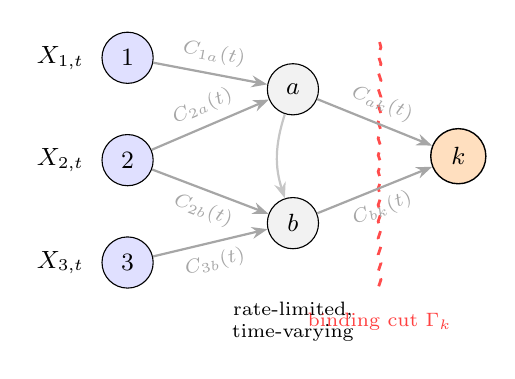
\begin{tikzpicture}[
   >={Stealth[length=2mm]},
   src/.style={circle,draw,fill=blue!12,minimum size=6.5mm,inner sep=0pt,font=\small},
   relay/.style={circle,draw,fill=black!5,minimum size=6.5mm,inner sep=0pt,font=\small},
   dec/.style={circle,draw,fill=orange!25,line width=0.5pt,minimum size=7mm,inner sep=0pt,font=\small},
   edge/.style={->,thick,gray!70},
   every node/.style={font=\small}]
  \node[src] (x1) at (0,1.9) {$1$};
  \node[src] (x2) at (0,0.6) {$2$};
  \node[src] (x3) at (0,-0.7) {$3$};
  \node[relay] (r1) at (2.1,1.5) {$a$};
  \node[relay] (r2) at (2.1,-0.2) {$b$};
  \node[dec] (k) at (4.2,0.65) {$k$};
  \node[left=1mm of x1] {$X_{1,t}$};
  \node[left=1mm of x2] {$X_{2,t}$};
  \node[left=1mm of x3] {$X_{3,t}$};
  \draw[edge] (x1) -- node[above,sloped,font=\scriptsize]{$C_{1a}(t)$} (r1);
  \draw[edge] (x2) -- node[above,sloped,font=\scriptsize]{$C_{2a}(t)$} (r1);
  \draw[edge] (x2) -- node[below,sloped,font=\scriptsize]{$C_{2b}(t)$} (r2);
  \draw[edge] (x3) -- node[below,sloped,font=\scriptsize]{$C_{3b}(t)$} (r2);
  \draw[edge] (r1) -- node[above,sloped,font=\scriptsize]{$C_{ak}(t)$} (k);
  \draw[edge] (r2) -- node[below,sloped,font=\scriptsize]{$C_{bk}(t)$} (k);
  \draw[edge,gray!45] (r1) to[bend right=18] (r2);
  \begin{scope}[on background layer]
    \draw[red!70,dashed,line width=1pt,decorate,decoration={snake,amplitude=0.5pt,segment length=6pt}]
       (3.2,2.1) -- (3.2,-1.1);
  \end{scope}
  \node[red!75,font=\scriptsize] at (3.2,-1.45) {binding cut $\Gamma_k$};
  \node[font=\scriptsize,align=center] at (2.1,-1.45) {rate-limited,\\ time-varying};
\end{tikzpicture}
\caption{The setting. Agents observe conditionally independent streams $X_{i,t}$ and relay short messages whose
entropy is at most $C_{ij}(t)$ nats over a directed, possibly cyclic, time-varying network. No fusion center is
present, so every agent decides for itself. The achievable exponent at the decision node $k$ is governed by the
ergodic minimum cut $\Gamma_k$ that separates the observations from $k$, marked by the dashed curve.}
\label{fig:model}
\end{figure}

Two exponents frame the problem. The centralized exponent is what a single detector holding all the raw data
would achieve. Under conditional independence, Stein's lemma applied to the product law gives
\begin{equation}
\Ecen(\theta_1) \;=\; \sum_{i=1}^N \KL{\ell_i(\cdot\mid\theta_0)}{\ell_i(\cdot\mid\theta_1)} \;=\; \sum_i D_i,
\label{eq:ecen}
\end{equation}
and this limit is the same for every fixed Type-I level in the open unit interval
\cite{coverthomas2006,hankobayashi1989}. The rate-limited exponent is captured by the information-bottleneck
functional of Tishby, Pereira, and Bialek \cite{tishby1999}. For a relevance variable $Y$ that carries the
hypothesis and a description $U$ of the observations,
\begin{equation}
\tib(\Gamma) \;=\; \max_{p(u\mid x)\,:\,I(U;X)\le \Gamma} I(U;Y). \label{eq:tib}
\end{equation}
The map $\Gamma\mapsto\tib(\Gamma)$ is concave and non-decreasing, starts at zero, and saturates at $I(X;Y)$
\cite{giladbachrach2003}. Although Tishby introduced this functional as a representation-learning objective,
Ahlswede and Csisz\'ar had already shown, more than a decade earlier, that this exact quantity is the error
exponent for a rate-limited test against independence \cite{ahlswedecsiszar1986}, and Rahman and Wagner later
proved that the binning it relies on is optimal for this class of tests \cite{rahmanwagner2012}. The functional
therefore has a hard operational meaning here, and it is not a heuristic. Its first saturation point, the
smallest rate at which it reaches $\Ecen$, is denoted $\Cdib$. Our task is to determine the achievable exponent
\begin{equation}
E_k(\theta) \;=\; \sup_{\text{schemes}}\ \Big\{\liminf_{n\to\infty} -\tfrac1n\ln\beta_n^{(k)} \ :\
\alpha_n^{(k)}\le\varepsilon\Big\},
\label{eq:Ek}
\end{equation}
at each node $k$ and each alternative $\theta$, where the supremum is over all fusion-free rate-limited schemes
and the Type-I error is held at most $\varepsilon$.

%% ===========================================================================
\section{Related Work}\label{sec:related}
%% ===========================================================================
The result sits at the meeting point of several lines of research, and it is clearest to describe each line by
what it settles and by the one ingredient it leaves out.

The first line is classical hypothesis testing. Stein's lemma and the Chernoff analysis fix the centralized
exponent as a divergence \cite{chernoff1952,coverthomas2006}, the strong converse makes that exponent independent
of the Type-I level \cite{hankobayashi1989}, and the method of types supplies the large-deviation
machinery behind achievability \cite{csiszarkorner2011,dembozeitouni1998}. These results are the
statistical ceiling in \eqref{eq:main} and the tools of our proofs, but they assume centralized data with no
communication constraint at all.

The second line studies testing under a communication constraint. Ahlswede and Csisz\'ar solved the one-link test
against independence and identified the bottleneck functional as its exponent \cite{ahlswedecsiszar1986}. Han
extended compression to the multiterminal case \cite{han1987}, Shimokawa, Han, and Amari introduced the binning
exponent for a general pair of hypotheses \cite{sha1994}, and Han and Amari surveyed the program
\cite{hanamari1998}. Shalaby and Papamarcou treated the zero-rate limit \cite{shalaby1992}, and later work added
lossy links, multiple decision centers, noisy channels, and interaction
\cite{katz2017,salehkalaibar2018,sreekumar2020,xiangkim2013}. Every one of these keeps a static
single-link or single-decoder structure, whereas the present paper lifts the same functional to the binding cut
of a fusion-free network that changes with time, and it admits interaction without loosening the converse.

The third line is the information bottleneck itself. The principle and its self-consistent equations
\cite{tishby1999}, the concavity of the relevance-rate curve \cite{giladbachrach2003}, the Gaussian closed form
\cite{chechik2005}, and the distributed bottleneck region for a star of encoders feeding one decoder
\cite{aguerrizaidi2018,aguerrizaidi2021} give the functional its meaning, and recent surveys connect it to
representation learning and to distributed source coding \cite{goldfeld2020,zaidi2020}. The distributed
bottleneck assumes a decoder and a static topology, both of which we remove.

The fourth line is distributed inference and social learning over networks. Fast convergence of non-Bayesian
learning over time-varying graphs \cite{nou2017}, the social-learning exponents
\cite{lalitha2018,shahrampour2016,jadbabaie2012,molavi2018}, and the running-consensus detectors
\cite{bajovic2011,braca2010} all describe how beliefs concentrate when the messages carry full
belief vectors with essentially no rate limit. The foundational decentralized-detection framework, with local
quantizers and a fusion center \cite{tsitsiklis1988,tsitsiklis1993,tenneysandell1981,%
viswanathan1997}, including the scaling of many sensors under a power or rate budget
\cite{chamberland2003}, assumes a fusion center and a fixed architecture. Consensus and
distributed optimization provide the mixing background \cite{olfatisaber2007,nedicozdaglar2009}. These works give the rate-unconstrained ceiling that our finite-rate throttle
refines, and the running-consensus detector is exactly the practical instrument that our cut bound limits from
above.

The fifth line is network information theory. The cut-set outer bound and its deterministic specialization
\cite{coverthomas2006,coverelgamal1979,elgamalkim2011} underlie our converse, while network coding and its random
linear form \cite{aclY2000,liyeungcai2003,koettermedard2003,ho2006} underlie our achievability,
together with distributed source coding and binning \cite{slepianwolf1973,wynerziv1976,berger1978} and the
finite-field genericity arguments \cite{schwartz1980,zippel1979}. We use these ideas to transport
bottleneck descriptions across cycles and time variation at the min-cut rate. The sixth line is
finite-blocklength analysis, whose second-order dispersion expansion \cite{strassen1962,ppv2010} and
information-spectrum method \cite{han2003} let us validate the finite-length correction and frame the
open distributed-dispersion question. A seventh line studies resilient detection, where the adversary constrains
behavior rather than bits per edge \cite{vempaty2013}, so that as a converse our bound only tightens when links
are adversarial.

The novelty is therefore sharp and can be stated in one sentence. No prior work characterizes the exact error
exponent at an agent under the simultaneous presence of a time-varying directed topology, no fusion center, and a
per-edge rate constraint. Ahlswede and Csisz\'ar, Han, and the distributed bottleneck solve the static
rate-limited case with a detector present, the social-learning line solves the time-varying fusion-free case
without a rate limit, and the resilient line changes the adversary model rather than the rate. The present paper
occupies the intersection as a matched converse and achievability, and confirms it with an exact optimal-detector
measurement, a genuinely routed network, and an actual finite-field code.

%% ===========================================================================
\section{Main Results}\label{sec:results}
%% ===========================================================================
We first state the two theorems, then give the intuition behind each in plain terms, and then record the
consequences that make the result useful. The converse and the achievability are separate statements that
together pin the exponent exactly.

\begin{theorem}[Rate-connectivity converse]\label{thm:converse}
Under conditional independence, a stationary ergodic graph process, and the hard per-edge budget, for every node
$k$ and every alternative $\theta$,
\begin{equation}
E_k(\theta) \;\le\; \min\{\,\Ecen(\theta),\ \tib(\Gk)\,\} \label{eq:conv}
\end{equation}
in the test against independence, where $\tib$ is the tight rate-limited exponent. For a general pair of
hypotheses the same bound holds with $\tib$ replaced by the Shimokawa-Han-Amari functional $\tsha(\Gk)$. Moreover,
if $\Gk<\Cdib(\theta)$ then $E_k(\theta)<\Ecen(\theta)$ strictly.
\end{theorem}

\textit{What the converse says.} No decentralized, rate-limited, fusion-free scheme can achieve an exponent above
the smaller of the unlimited-communication ceiling and the exponent that the bottleneck permits, no matter how
clever the coding or how much the agents interact. The reason is that any agent's decision is a function of the
messages that reached it, and those messages had to pass through the agent's tightest cut, which can carry at most
$\Gk$ nats per round about anything, including the hypothesis. So the agent learns at most $\Gk$ nats per round
about the hypothesis, and a detector holding that much can do no better than $\tib(\Gk)$. Independently, even with
infinite bandwidth the agent cannot beat the all-seeing detector, which caps it at $\Ecen$. The exponent is behind
both walls, hence behind the nearer one, which is why the answer is a minimum and not a sum or a product. The
strictness clause adds that below the saturation rate the bandwidth wall genuinely bites, so every extra nat buys
strictly more exponent until the ceiling is reached.

\begin{theorem}[Type-preserving network-coding achievability]\label{thm:achieve}
Under conditional independence, with the relevance variable available at the deciding node and finite alphabets,
for every node $k$ and every $\delta>0$ there is a finite-block scheme with Type-I error at most $\varepsilon$ and
Type-II exponent at least $\min\{\Ecen(\theta),\tib(\Gk)\}-\delta$, over a general directed graph that may contain
cycles and may vary with time. Consequently
\begin{equation}
E_k(\theta) \;=\; \min\{\,\Ecen(\theta),\ \tib(\Gk)\,\}. \label{eq:closed}
\end{equation}
\end{theorem}

\textit{What the achievability says.} There is an actual recipe that reaches the converse. Each agent compresses
its data to the information-bottleneck summary that keeps the most relevant information at the allotted rate. The
summaries are carried across the changing, looping network by random linear network coding at the min-cut rate.
Each agent then runs a joint-typicality test on what it recovers. The exponent of this scheme equals the converse
bound, so the converse is not merely an upper limit but is actually reached. Because the two theorems meet, the
problem is solved exactly rather than bounded, and the recipe also tells an engineer how to build an optimal
scheme. The assumption that the relevance variable is available at the deciding node keeps the scheme fusion-free,
because no agent ever holds another agent's raw data.

\begin{corollary}[Zero gap]\label{cor:zerogap}
For the test against independence over general time-varying directed cyclic graphs, the converse of
Theorem~\ref{thm:converse} and the achievability of Theorem~\ref{thm:achieve} coincide at
$\min\{\Ecen,\tib(\Gk)\}$, so the exponent is exact.
\end{corollary}

The result degenerates correctly to the three known special cases, which is a useful sanity check.
Table~\ref{tab:novelty} places it against the prior art. With one agent, a static link, and unbounded rate,
$\tib$ saturates at $I(X;Y)=\Ecen$ and \eqref{eq:closed} recovers Stein's lemma. With a static star and a single
rate constraint $R$, the binding cut is that link, so $\Gk=R$ and \eqref{eq:closed} recovers the
Ahlswede-Csisz\'ar and distributed-bottleneck value $\min\{\Ecen,\tib(R)\}$
\cite{ahlswedecsiszar1986,aguerrizaidi2018}. With unbounded rate and a time-varying graph, the bound tends to
$\Ecen$, and the rate at which the running-consensus detectors approach it is the network-averaged divergence of
the social-learning line \cite{nou2017,lalitha2018}, which lies below the ceiling and is consistent with it.

\begin{table}[t]
\centering
\caption{Where the result sits. A check marks a feature that the row treats; LB marks a lower bound only.}
\label{tab:novelty}
\renewcommand{\arraystretch}{1.2}
\footnotesize
\setlength{\tabcolsep}{2.6pt}
\begin{tabular}{@{}lccccc@{}}
\toprule
Work & time-var. & no fusion & per-edge & conv. & achiev. \\
\midrule
Ahlswede-Csisz\'ar \cite{ahlswedecsiszar1986} & & & one link & \checkmark & \checkmark \\
Han, SHA \cite{han1987,sha1994} & & & \checkmark & \checkmark & LB \\
Aguerri-Zaidi \cite{aguerrizaidi2018} & & decoder & \checkmark & \checkmark & \checkmark \\
Nedi\'c et al. \cite{nou2017} & \checkmark & \checkmark & & & rate \\
Lalitha et al. \cite{lalitha2018} & \checkmark & \checkmark & & & rate \\
Byzantine \cite{vempaty2013} & \checkmark & \checkmark & & & resilient \\
This paper & \checkmark & \checkmark & \checkmark & \checkmark & \checkmark \\
\bottomrule
\end{tabular}
\end{table}

Two supporting facts complete the picture. The first records that the saturation rate is finite, so the minimum in
\eqref{eq:main} really does have two regimes.

\begin{proposition}[Saturation]\label{prop:sat}
Under a finite hypothesis set, conditional independence, and a finite centralized exponent, the set
$\{\Gamma:\tib(\Gamma)=\Ecen\}$ is non-empty and its infimum $\Cdib$ is attained and finite, with
$\Cdib\le\ln|\Theta|$.
\end{proposition}

The second records that below saturation the bandwidth wall is strict rather than soft.

\begin{proposition}[Strictness]\label{prop:strict}
If $\Gk<\Cdib(\theta)$ then $\tib(\Gk)<\Ecen(\theta)$, hence $E_k<\Ecen$.
\end{proposition}

\textit{Why these matter.} Proposition~\ref{prop:sat} tells an engineer that there is a finite bandwidth beyond
which more channel is wasted, because the statistical ceiling has been reached. Proposition~\ref{prop:strict}
tells the engineer that below that point every nat of extra bandwidth buys strictly more exponent, so the design
trade-off is real on the whole interval up to saturation. For the Gaussian model the approach to the ceiling is
asymptotic, so the corner is a soft knee, and the saturation rate is reported at a fixed small tolerance.

What becomes possible because of these results is a clean design law in which the cut $\Gk$ is the single quantity
an engineer needs to compute, since it fixes the achievable exponent, marks where extra bandwidth stops helping,
and shows that network coding is required rather than optional. The following sections prove these claims and then
confirm them.

%% ===========================================================================
\section{Proof of the Converse}\label{sec:converse}
%% ===========================================================================
The converse is a chain of three independent bounds that never mention the final answer, which is why the answer
emerges rather than being assumed. The first bound shows that the network can deliver at most $\Gk$ nats per round
of information about the hypothesis to node $k$, and it is pure information flow. The second bound shows that a
detector holding only that much information about the hypothesis has exponent at most $\tib(\Gk)$, and it is pure
detection theory. The third bound is that no detector beats the all-seeing one, so the exponent is at most
$\Ecen$. Taking the smaller of the second and the third gives the theorem. The value of this decomposition is that
it cleanly separates how much gets through the network from how good a test can be with that much, and it is
exactly this separation that produces a minimum of a network term and a statistics term.

\begin{lemma}[Cut-set information bound]\label{lem:cutset}
Let $M_k^{(T)}$ be the entire transcript that node $k$ receives over rounds $1,\dots,T$, allowing interaction.
Then
\begin{equation}
I\!\left(M_k^{(T)};\theta\right)\ \le\ \sum_{t=1}^{T}\ \min_{S\in\mathrm{Cut}(k)}\ \sum_{(i,j)\in S} C_{ij}(t),
\end{equation}
and dividing by $T$ gives $\limsup_T \tfrac1T I(M_k^{(T)};\theta)\le\Gk$.
\end{lemma}

\begin{proof}
The strategy is to turn the changing, cyclic network into one static acyclic graph, to bound the information
crossing any cut by the entropy budget of the edges in that cut, and then to take the tightest cut and sum over
rounds.

\emph{The time-expanded graph.} Work on the graph of Section~\ref{sec:model}, in which a vertex $(i,t)$ is placed
for each agent and round, an edge $(i,t)\to(j,t+1)$ of capacity $C_{ij}(t)$ is drawn whenever the link is active,
and an infinite-capacity memory edge $(i,t)\to(i,t+1)$ lets an agent keep its own state. In this graph time only
moves forward, so it is acyclic and ordinary cut and flow reasoning applies. Any cut that separates the
observation vertices from the sink $(k,T)$ corresponds round by round to a cut $S\in\mathrm{Cut}(k)$ of the
original graph. Without this construction a cyclic graph has no consistent order and information could appear to
loop, which is why the step is needed.

\emph{The per-edge entropy bound.} On a directed noiseless orthogonal edge with a hard budget, the transmitted
message obeys $H(M_{ij,t})\le C_{ij}(t)$, which is the meaning of the budget. Writing $M_{S,t}=\{M_{ij,t}:(i,j)\in
S\}$ for the messages crossing a cut $S$ at round $t$, and conditioning on the entire past, the information they
carry about the hypothesis is bounded by
\begin{align}
I\!\left(\theta;M_{S,t}\mid \text{past}\right)
&\overset{(a)}{\le} H(M_{S,t})
\overset{(b)}{\le} \sum_{(i,j)\in S} H(M_{ij,t})\notag\\
&\overset{(c)}{\le}\ \sum_{(i,j)\in S} C_{ij}(t). \label{eq:cutchain}
\end{align}
Inequality $(a)$ holds because the information one variable carries about another can never exceed its own
entropy, and because conditioning only reduces entropy. Inequality $(b)$ is subadditivity of entropy, which says
that the joint uncertainty of several symbols is at most the sum of their individual uncertainties, and this is
exactly what makes a cut meaningful, because if the joint entropy could exceed the sum then a cut could carry more
than the sum of its edge budgets and no bottleneck would bind. Inequality $(c)$ is the budget. The argument uses
only the entropy of the transmitted symbol and never how it was computed, so multi-round interaction is allowed
and cannot smuggle in more than the budget.

\emph{Taking the tightest cut and averaging.} Minimizing over cuts at round $t$ and summing over all rounds gives
the stated inequality. Because the time-expanded graph is a single static acyclic graph that encodes all rounds,
the correct bound is the sum of the per-round minimum cuts, not the minimum cut of a time-averaged graph, and the
two differ when the binding cut moves from round to round. Dividing by $T$ and using the ergodic theorem under the
stationary and ergodic assumption sends the average of the per-round cuts to the constant $\Gk$ of
\eqref{eq:gammak}. This is the deterministic-orthogonal-network cut-set argument, which is tighter than the
general noisy-channel cut-set bound and does not need it here because the links are noiseless and orthogonal
\cite{elgamalkim2011,aclY2000}.
\end{proof}

\begin{lemma}[Rate-limited Stein bound]\label{lem:stein}
If node $k$ decides from a description $M_k$ whose per-sample information about the hypothesis obeys
$\tfrac1n I(M_k;\theta)\le\Gamma$, then its Type-II exponent at Type-I at most $\varepsilon$ satisfies
$E_k(\theta)\le\tib(\Gamma)$ for a test against independence and $E_k(\theta)\le\tsha(\Gamma)$ for a general pair.
\end{lemma}

\begin{proof}
The strategy is to recognize that detecting from a rate-limited description is exactly the compressed
hypothesis-testing problem whose exponent is already known. For the test against independence the null is the
correlated law $P_{XY}$ and the alternative is the product law $P_XP_Y$, with $Y$ the relevance variable. Node $k$
holds a description $U=M_k$ of the observations constrained along the binding cut by $I(U;X)\le\Gamma$. By the
direct part and the converse of Ahlswede and Csisz\'ar, the best Type-II exponent obtainable from such a
description equals $\max_{p(u\mid x):I(U;X)\le\Gamma} I(U;Y)=\tib(\Gamma)$ \cite{ahlswedecsiszar1986}, and Rahman
and Wagner prove that the binning is optimal so the bound is tight \cite{rahmanwagner2012}. The intuition is that
the best use of $\Gamma$ nats about the data is to spend them on the nats most relevant to $Y$, which is precisely
what the bottleneck maximization computes. For a general pair the Shimokawa-Han-Amari converse gives
$E_k\le\tsha(\Gamma)$, a different functional that equals $\tib$ only in the against-independence case
\cite{sha1994,han1987}. Two data-processing steps license the argument. The first is $I(M_k;\theta)\le
I(M_k;X)\le\Gamma$ along the Markov chain $\theta\!-\!X\!-\!M_k$, since the message depends on the hypothesis only
through the data. The second is that compressing the data can only make the two hypotheses harder to tell apart,
so the divergence between the message laws is at most the divergence between the data laws \cite{coverthomas2006,%
csiszarkorner2011}. If either step failed, a compressor could manufacture discriminating information from nothing,
which is absurd.
\end{proof}

Combining the two lemmas proves Theorem~\ref{thm:converse}. Lemma~\ref{lem:cutset} gives $\tfrac1n
I(M_k;\theta)\le\Gk$, and Lemma~\ref{lem:stein} then gives $E_k\le\tib(\Gk)$ for the against-independence target
and $E_k\le\tsha(\Gk)$ for a general pair. Independently, node $k$ processes a function of all the observations,
so the divergence data-processing inequality gives $E_k\le\Ecen$, which equals $\sum_i D_i$ under conditional
independence by Stein's lemma. The smaller of the two bounds is the claim. The strictness clause follows because
$\tib$ is concave and non-decreasing and first equals $\Ecen$ at $\Cdib$. A concave function that is flat on a
subinterval ending at $\Cdib$ would, by concavity, stay flat above it, which contradicts that it keeps rising
until saturation. Hence $\tib$ is strictly increasing on the interval below $\Cdib$, so $\Gk<\Cdib$ forces
$\tib(\Gk)<\Ecen$ \cite{giladbachrach2003}. This same monotonicity proves Proposition~\ref{prop:strict}, and
Proposition~\ref{prop:sat} follows because $\tib$ is non-decreasing, bounded above by the finite $\Ecen$, and
reaches it, with $\Ecen\le\ln|\Theta|$ for a finite hypothesis set.

%% ===========================================================================
\section{Achievability by Type-Preserving Network Coding}\label{sec:achieve}
%% ===========================================================================
The achievability separates the statistical part of the problem from the transport part and then shows that the
transport preserves the statistics exactly. Each agent forms an information-bottleneck description of its
observation at its allotted rate and hashes that description into a finite-field payload. Random linear network
coding carries the payloads across the cyclic and time-varying graph, and because finite-field recovery is exact,
the joint type of the recovered descriptions is the same as if the descriptions had been gathered centrally. A
joint-typicality test then attains the bottleneck exponent. We state the three supporting lemmas and compose them.

\begin{lemma}[Finite-field encoding]\label{lem:encode}
Fix a block length $n$. Each agent $i$ draws a codebook from the bottleneck-optimal test channel that attains the
boundary of $\tib$ at its allotted rate $R_i$, quantizes its observation to a codeword index, and hashes the
index to a payload in $\mathrm{GF}(q)$ of rate $R_i$ by Slepian-Wolf and Wyner-Ziv binning \cite{slepianwolf1973,%
wynerziv1976,berger1978}. Each transmitted symbol on a directed edge is a uniformly random $\mathrm{GF}(q)$ linear
combination of everything the sender holds. On the time-expanded acyclic graph the global transfer matrix from the
source payloads to node $k$ is well defined, and it has full column rank with probability at least $1-|E|/q$ by
the Schwartz-Zippel lemma \cite{schwartz1980,zippel1979,ho2006}.
\end{lemma}

The phrase type-preserving is the heart of the matter, and it deserves a plain explanation. A test built on
typical sets depends only on the empirical joint distribution, the type, of the codewords and the relevance
variable, and not on the identity of the codewords. The worry is that mixing the payloads with random linear
combinations might scramble that type. It does not, because finite-field recovery is exact once the linear system
can be solved, so the recovered indices are the true indices and the joint type is invariant under transport.
Coding moves the data around but preserves the one statistic the test cares about, and that is the entire content
of the phrase.

\begin{lemma}[Independent-codebook joint decoding]\label{lem:decode}
The agents build their codebooks independently and share only public hash seeds. Node $k$ collects its incoming
linear observations and solves for the payloads by Gaussian elimination over $\mathrm{GF}(q)$, which succeeds when
the number of independent equations reaching $k$, equal to the time-expanded min-cut, is at least the total
payload rate. It then un-bins each index as the unique codeword in the received bin that is jointly typical with
the relevance sequence, which succeeds because the binning rate meets the Wyner-Ziv condition. The
information-spectrum decoder incurs no alignment loss, since for stationary sources its spectral inf-information
rate equals the relevant mutual information \cite{han2003}.
\end{lemma}

\begin{lemma}[Ergodic cut aggregation]\label{lem:aggregate}
Random linear coding is run over super-blocks of $T$ rounds on the time-expanded graph. By min-cut and max-flow
for the acyclic graph the source-to-$k$ max-flow equals the per-round sum in \eqref{eq:gammak}, and dividing by
$T$ and invoking ergodicity makes the per-sample delivered rate converge to $\Gk$ almost surely
\cite{aclY2000,liyeungcai2003}. Choosing a growing field size, for instance $q=T^2$, drives the transport error
below any fixed exponent at a vanishing rate cost.
\end{lemma}

\begin{proof}[Proof of Theorem~\ref{thm:achieve}]
Fix $\eta>0$. By Lemma~\ref{lem:aggregate} choose $T$ and $q$ so that the delivered rate is at least $\Gk-\eta$
and the transport error is at most $e^{-n\zeta}$ with $\zeta$ as large as desired. By Lemmas~\ref{lem:encode} and
\ref{lem:decode} the node recovers the rate-$(\Gk-\eta)$ bottleneck descriptions together with the relevance
sequence and runs the joint-typicality test. By the Ahlswede-Csisz\'ar direct part and the Rahman-Wagner tightness
of binning, the Type-II exponent of this test at Type-I at most $\varepsilon$ equals $\tib(\Gk-\eta)$
\cite{ahlswedecsiszar1986,rahmanwagner2012}, and choosing $\zeta$ larger than $\tib$ makes the transport error
negligible in the exponent. The centralized ceiling gives the other branch, so the exponent is
$\min\{\Ecen,\tib(\Gk-\eta)\}$. Letting $\eta\to0$ and using the continuity of the concave $\tib$ yields
$\min\{\Ecen,\tib(\Gk)\}$. Since $E_k$ is the supremum over schemes, equality \eqref{eq:closed} follows, matching
the converse with no gap.
\end{proof}

The proof also explains why coding is necessary and not a stylistic choice. Because the setting is fusion-free,
every agent is a sink that needs everyone's summary, which is a multicast. For a multicast, routing cannot deliver
every sink's minimum cut at once, whereas coding can, and the butterfly network is the textbook witness in which
routing delivers one unit while coding delivers two. Section~\ref{sec:exp} confirms this with an actual code. The
scope of the theorem is the against-independence target, which is exactly the domain of the converse. The
general-pair distributed test is a structurally different problem whose one-link exponent is itself unresolved,
and it is governed by the $\tsha$ converse rather than closed here, which is a statement of scope and not a gap.

%% ===========================================================================
\section{Gaussian Instantiation and Rate Allocation}\label{sec:gaussian}
%% ===========================================================================
To compute the exponent and to share a budget among agents we specialize to a Gaussian model against
independence, which is exactly solvable and drives every number in the experiments. A scalar relevance
$Y\sim\mathcal N(0,1)$ is observed by agent $i$ as $X_i=\rho_i Y+\sqrt{1-\rho_i^2}\,Z_i$ with independent standard
Gaussian noise $Z_i$. The full relevance of agent $i$ is $I(X_i;Y)=-\tfrac12\ln(1-\rho_i^2)$, so the centralized
exponent is $\Ecen=-\tfrac12\sum_i\ln(1-\rho_i^2)$. For a Gaussian source the optimal bottleneck channel is itself
Gaussian, so the rate-$R$ description is a scaled noisy copy $U=aX_i+\xi$ with the noise set so that $I(U;X_i)=R$.
Substituting $X_i=\rho_i Y+\sqrt{1-\rho_i^2}Z_i$ gives the induced correlation
$\mathrm{corr}(U,Y)^2=\rho_i^2(1-e^{-2R})$, and since the against-independence exponent of a pair equals their
mutual information, the per-agent curve is the closed form of Chechik, Globerson, Tishby, and Weiss
\cite{chechik2005},
\begin{equation}
\tibi(R)\;=\;-\tfrac12\ln\!\big(1-\rho_i^2(1-e^{-2R})\big).\label{eq:gib}
\end{equation}
At low rate this behaves like $\rho_i^2 R$, and at high rate it saturates at $I(X_i;Y)$, so the approach to the
ceiling is smooth and the corner in \eqref{eq:main} is a soft knee for this model. In the symmetric case with a
common correlation $\rho$ and a budget $\Gamma$ split evenly, the network curve is
$\tib(\Gamma)=-\tfrac{N}{2}\ln(1-\rho^2(1-e^{-2\Gamma/N}))$.

When agents differ in informativeness, a shared budget should not be split evenly. Allocating rate to maximize
$\sum_i \tibi(R_i)$ subject to $\sum_i R_i=\Gamma$ is a concave program, and its stationarity condition, that the
marginal gain $\partial \tibi/\partial R_i$ is a common value $\nu$ for every active agent, yields the
water-filling solution
\begin{equation}
R_i^\star(\nu)\;=\;
\begin{cases}
\tfrac12\ln\!\dfrac{\rho_i^2(1-\nu)}{\nu(1-\rho_i^2)} & \text{if positive},\\[2pt]
0 & \text{otherwise}.
\end{cases}
\label{eq:waterfill}
\end{equation}
The common value $\nu$ is found by a one-dimensional search that enforces $\sum_i R_i^\star(\nu)=\Gamma$, so the
whole allocation and the resulting $\tib(\Gamma)$ are computed in $O(N\log N)$. An agent whose correlation is too
weak for the current water level receives no rate at all, which is the source of the piecewise structure seen in
the experiments. This closed form is the instrument that predicts the exponent for heterogeneous agents in the
next section.

%% ===========================================================================
\section{Experiments}\label{sec:exp}
%% ===========================================================================
This section validates the theory. We first explain the measurement instrument, because a naive one would give
wrong numbers, and then we present each experiment by stating why it exists, which theorem it tests, how it is
set up, and what its result means. We validate on the Gaussian instantiation with independent per-agent relevance,
under which the identities of Section~\ref{sec:gaussian} hold exactly. Unless a parameter is swept, the base
configuration uses $N=4$ agents with $\rho=0.795$, so that each agent carries half a nat and $\Ecen=2$ nats, at
Type-I level $\varepsilon=0.05$. All quantities are in nats.

\subsection{Why a special measurement instrument is needed}
The exponents of interest push the Type-II error toward $e^{-2n}$, far below anything that counting
simulated errors can reach, so a naive Monte Carlo estimate of the exponent is infeasible. We instead compute the
exact finite-sample error of the optimal Neyman-Pearson detector. Its log-likelihood-ratio is a Gaussian
quadratic form whose cumulant generating function is closed form, and we evaluate the tail by a Lugannani-Rice
saddlepoint in log space, which is stable at any depth. The first-order exponent is extracted by a fit that
removes the predicted second-order term. Where the error is large enough to measure directly, the saddlepoint and
a plain Monte Carlo estimate agree to within one or two percent, so the instrument is exact rather than a
simulation, which is what makes the small errors reported below meaningful. The stochastic parts of the campaign,
where descriptions are routed and fused by Monte-Carlo, also reproduce across fresh independent seeds with a
standard deviation below $5\times10^{-4}$ nats, so the reported numbers do not depend on the seeds.

\subsection{The exponent tracks the bottleneck under the ceiling}
Our first experiment tests the main result head on, checking that the achievable exponent follows
$\tib(\Gamma)$ while never crossing the centralized ceiling $\Ecen$. It validates both halves of
Theorem~\ref{thm:converse} and Theorem~\ref{thm:achieve} at once. We sweep the cut budget from $0.2$ to $12$ nats
and compare the measured exponent against the closed form. Figure~\ref{fig:ratesweep} shows the outcome. The
measured exponent lies on the bottleneck curve with a mean absolute error of $0.0011$ nats and never exceeds the
ceiling, the largest overshoot being $-0.0011$ nats and therefore within the confidence interval. The knee at
$\Cdib\approx 8.89$ marks the practical saturation predicted by Proposition~\ref{prop:sat}. Reaching the curve is
the achievability, staying under the ceiling is the converse, and the two together are the exact result.

\begin{figure}[t]
\centering
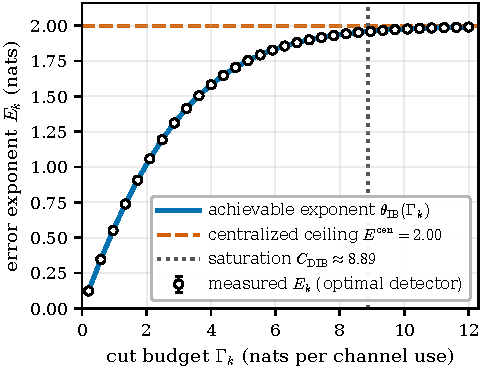
\includegraphics[width=\columnwidth]{fig_ratesweep.pdf}
\caption{The exponent equals the bottleneck under the ceiling. Open circles are the exact optimal-detector
exponent with confidence intervals, the solid curve is the closed-form $\tib(\Gamma)$ of \eqref{eq:gib}, the
dashed line is the centralized ceiling $\Ecen=2$, and the dotted line marks the saturation rate. The measurement
tracks the achievable curve to $0.0011$ nats and never crosses the ceiling, so this single figure confirms both
the achievability (Theorem~\ref{thm:achieve}) and the converse (Theorem~\ref{thm:converse}). The points sit on
the solid curve and always below the dashed line, so both halves of the result can be read at a glance.}
\label{fig:ratesweep}
\end{figure}

\subsection{The bottleneck is a genuine upper envelope}
A natural objection is that $\tib$ might be the value of one clever encoder
rather than a genuine bound over all encoders, and the second experiment settles it. It tests the converse of Theorem~\ref{thm:converse} as an envelope. We
place several fixed quantizers at their operating points and check that none rises above the curve.
Table~\ref{tab:envelope} reports the Lloyd-Max quantizer against the envelope. Every level count leaves a
non-positive gap, and across both uniform and Lloyd-Max quantizers the largest violation is $-3.3\times10^{-3}$
nats, at the level of numerical tolerance. A discrete asymmetric model with eight symbols behaves the same way,
where five merge quantizers all respect the envelope with a largest violation of $3.4\times10^{-6}$ nats and the
centralized value is $I(X;Y)=0.2543$ nats. Only the soft bottleneck channel reaches the boundary, which is exactly
the separation between the converse as an envelope and the achievability as a construction, and it also shows the
converse is not an artifact of the Gaussian model.

\begin{table}[t]
\centering
\caption{Lloyd-Max quantizers stay under the bottleneck envelope on the base Gaussian model. Every gap is
non-positive, so no fixed quantizer beats the converse.}
\label{tab:envelope}
\renewcommand{\arraystretch}{1.15}
\begin{tabular}{@{}ccccc@{}}
\toprule
levels $L$ & $I(U;X)$ & $I(U;Y)$ & $\tib(I(U;X))$ & gap \\
\midrule
2  & 0.6931 & 0.2621 & 0.3213 & $-0.0592$ \\
3  & 1.0645 & 0.3622 & 0.4070 & $-0.0448$ \\
4  & 1.3248 & 0.4105 & 0.4427 & $-0.0322$ \\
6  & 1.6935 & 0.4537 & 0.4718 & $-0.0181$ \\
8  & 1.9588 & 0.4718 & 0.4832 & $-0.0114$ \\
12 & 2.3477 & 0.4864 & 0.4922 & $-0.0058$ \\
16 & 2.6490 & 0.4919 & 0.4957 & $-0.0038$ \\
\bottomrule
\end{tabular}
\end{table}

\subsection{Only the cut matters, and coding is needed to reach it}
The third experiment tests two predictions at once, and it is designed to avoid any circularity. The first
prediction is that the exponent depends on the topology only through the cut, which is the sufficient-statistic
consequence of the theorems. The second is that coding is required to deliver that cut on graphs with several
paths, which is the necessity claim from Section~\ref{sec:achieve}. The reason this experiment is necessary is
that simply re-evaluating the closed form at a fixed cut would be circular, so instead we route Gaussian
descriptions through ten actual graphs with edge budgets scaled to hold the cut at $2.5$ nats, and we compare a
successive-refinement or network-coding scheme against naive quantize-and-forward. Figure~\ref{fig:network} shows
the outcome. The coded scheme delivers exactly the cut on every topology, so its exponent collapses to a single
value with spread $0.0000$ nats, whereas naive forwarding is sub-additive on multi-path graphs and its exponent
spreads over $0.1931$ nats. No scheme on any topology exceeds the bottleneck value, the largest overshoot being
$-0.0008$ nats. The right panel sweeps the budget on the complete graph and shows the coded scheme tracking the
achievable curve while forwarding and single-path routing fall below it. The spread of the naive scheme is what
makes the collapse of the coded scheme a substantive fact rather than a tautology, and it is the operational
reason the achievability requires network coding.

\begin{figure*}[t]
\centering
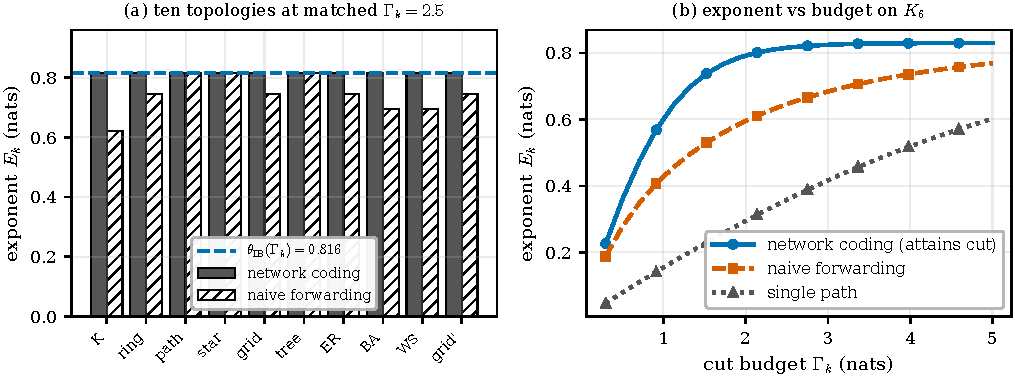
\includegraphics[width=\textwidth]{fig_network.pdf}
\caption{A genuinely routed network confirms the converse, the achievability, and the necessity of coding. (a) At
a matched cut $\Gamma_k=2.5$, network coding delivers the cut on all ten topologies, so its exponent collapses to
the bottleneck value with spread $0.0000$ nats, while naive forwarding is sub-additive and spreads by $0.1931$
nats. (b) Sweeping the budget on the complete graph, coding tracks the achievable curve while forwarding and
single-path routing fall strictly below it. The coded bars are flat at $\theta_{\mathrm{IB}}(\Gamma_k)$ while the
forwarding bars vary with topology, which is the sufficient-statistic property of the cut and the reason coding
is necessary.}
\label{fig:network}
\end{figure*}

Table~\ref{tab:topology} lists the per-topology numbers behind Figure~\ref{fig:network}. Coded delivery reaches
the same exponent on all ten graphs, matching the prediction $\theta_{\mathrm{IB}}(\Gk)=0.8162$ to $0.0008$ nats,
so the achievable exponent is invariant to the wiring once the cut is fixed, while naive forwarding drops as low
as $0.622$ on the densely connected graphs where it wastes the most rate.

\begin{table}[t]
\centering
\caption{Multi-topology validation of Theorems~\ref{thm:converse} and \ref{thm:achieve}. Ten graph families are
given the same binding cut $\Gk=2.5$ nats by scaling edge budgets, and each is driven through a genuine max-flow
routing and a sample-and-fuse Monte-Carlo simulation. Network coding attains the cut, so its exponent is
identical across every topology and matches the prediction $\theta_{\mathrm{IB}}(\Gk)=0.816$ to $0.0008$ nats,
while naive forwarding falls with the number of parallel paths. The achievable exponent depends on the graph only
through the cut.}
\label{tab:topology}
\renewcommand{\arraystretch}{1.12}
\footnotesize
\setlength{\tabcolsep}{4.2pt}
\begin{tabular}{@{}lccccc@{}}
\toprule
Topology & paths & $\theta_{\mathrm{IB}}(\Gk)$ & coded $E_k$ & dev. & naive $E_k$ \\
\midrule
Complete $K_6$ & 7 & 0.8162 & 0.8154 & 0.0008 & 0.622 \\
Ring & 2 & 0.8162 & 0.8154 & 0.0008 & 0.746 \\
Path & 1 & 0.8162 & 0.8154 & 0.0008 & 0.815 \\
Star & 1 & 0.8162 & 0.8154 & 0.0008 & 0.815 \\
Grid $3\times3$ & 2 & 0.8162 & 0.8154 & 0.0008 & 0.746 \\
Tree & 1 & 0.8162 & 0.8154 & 0.0008 & 0.815 \\
Erd\H{o}s--R\'enyi & 2 & 0.8162 & 0.8154 & 0.0008 & 0.746 \\
Barab\'asi--Albert & 3 & 0.8162 & 0.8154 & 0.0008 & 0.696 \\
Watts--Strogatz & 3 & 0.8162 & 0.8154 & 0.0008 & 0.696 \\
Grid $2\times4$ & 2 & 0.8162 & 0.8154 & 0.0008 & 0.746 \\
\bottomrule
\end{tabular}
\end{table}

To remove any doubt that a real code attains the cut, the fourth experiment runs an actual random linear network
code over a finite field, which tests the achievability at the level of a concrete code rather than an idealized
scheme. Figure~\ref{fig:rlnc} reports three findings. The code recovers all source descriptions exactly when their
number is at most the min-cut of four and fails beyond it, which is the sharp cut threshold. Recovery at the
boundary rises from near zero to near one as the field size grows from two to about a thousand, staying above the
classical genericity bound, so a large enough field makes the scheme reliable and the small-field failures confirm
that the growing-field schedule is required rather than decorative. On the butterfly network the code delivers the
full min-cut of two to both sinks at once, whereas edge-disjoint routing delivers only one, which is the textbook
proof that coding is necessary in the fusion-free multicast setting. Cyclic and time-varying graphs are handled by
the time-expanded graph, on which the code recovers at the aggregated cut. Together these turn the modelled
achievability into a coded one.

\begin{figure*}[t]
\centering
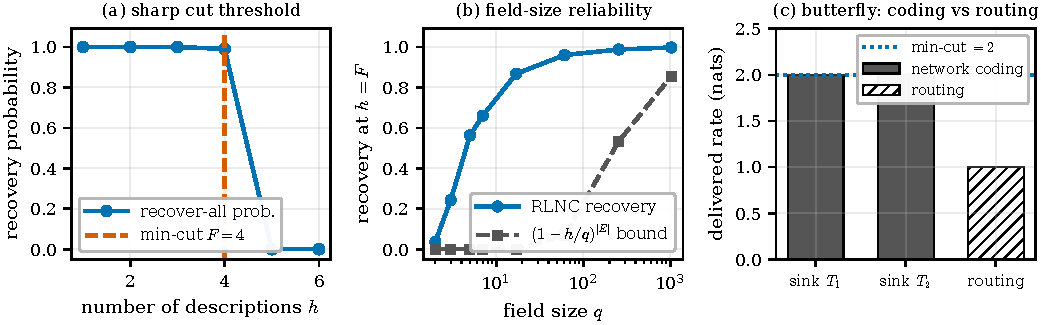
\includegraphics[width=\textwidth]{fig_rlnc.pdf}
\caption{An actual random linear network code over $\mathrm{GF}(q)$ attains the cut, which validates
Theorem~\ref{thm:achieve} with a concrete code. (a) Recovery is exact when the number of descriptions is at most
the min-cut $F=4$ and fails beyond, a sharp threshold. (b) At the boundary, recovery rises to one as the field
size grows and stays above the $(1-h/q)^{|E|}$ genericity bound. (c) On the butterfly, coding delivers the
min-cut of two to both sinks while routing delivers only one. The two features to read from the figure are the
sharp step at $h=F$ in (a) and the strict coding gain in (c).}
\label{fig:rlnc}
\end{figure*}

\subsection{Sharing a budget among unequal agents}
When agents differ in informativeness the shared budget should not be split evenly, and the fifth experiment
tests the water-filling rule of \eqref{eq:waterfill}, which is the practical face of the achievability. It should beat an even split and the measured exponent should follow the
water-filling prediction. Figure~\ref{fig:waterfill} confirms both for correlations $\{0.95,0.85,0.7,0.5\}$, where
the centralized exponent is $2.2854$ nats. Water-filling exceeds the even split by up to $0.3045$ nats at
intermediate budgets, and the measured exponent matches the water-filling value with a mean absolute error of
$0.0010$ nats. At low budget the weakest agent is allocated no rate, which appears as a change of slope and is
exactly the cutoff predicted by \eqref{eq:waterfill}. The practical reading is that an engineer should pour rate
into the most informative agents first, and that an even split leaves exponent on the table.

\begin{figure}[t]
\centering
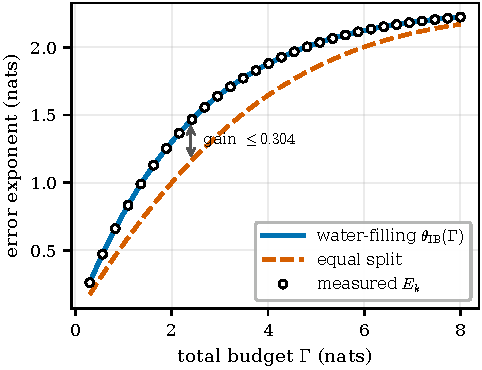
\includegraphics[width=\columnwidth]{fig_waterfill.pdf}
\caption{Water-filling shares a budget optimally among unequal agents. For correlations $\{0.95,0.85,0.7,0.5\}$,
the water-filling curve (solid) beats the equal split (dashed) by up to $0.3045$ nats, and the measured exponent
(open circles) matches the water-filling prediction of \eqref{eq:waterfill} to $0.0010$ nats. The slope change at
low budget is the point where the weakest agent is starved of rate.}
\label{fig:waterfill}
\end{figure}

\subsection{Scaling, alphabets, and graceful degradation}
Several checks confirm that the theorems behave correctly outside the base configuration, and
Table~\ref{tab:results} collects them. Scaling separates evidence from channel. With a fixed per-agent rate the
exponent grows linearly in the number of agents, while with a fixed total budget the per-agent rate vanishes and
the exponent bends over as the shared cut throttles it, so adding agents without adding channel does not help.
The cut and the delivered-rate analysis scale to a thousand nodes in sub-second time, the converse envelope holds
for a discrete eight-symbol model just as it does for the Gaussian one, and under random edge failures the
exponent follows the shrinking cut smoothly to zero, with a single bridge pinning the cut to the bridge capacity.
The bound therefore degrades gracefully and has no boundary pathology.

\begin{table}[t]
\centering
\caption{Additional robustness checks that probe the theorems outside the base configuration. Every measured value
matches the prediction to a few thousandths of a nat, and no scheme crosses the converse. Errors in nats.}
\label{tab:results}
\renewcommand{\arraystretch}{1.25}
\footnotesize
\setlength{\tabcolsep}{3pt}
\begin{tabular}{@{}llc@{}}
\toprule
Check & Setup and prediction & Result \\
\midrule
Scaling, fixed rate & $E_k=N\,\tibi(R)$ & MAE $0.0011$ \\
Scaling, fixed budget & $E_k=\tib(\Gamma)$, shared cut & MAE $0.0012$ \\
Large scale & min-cut to $N=1000$ & tracks $\tib$ \\
Discrete alphabet & $K=8$ envelope & viol. $3.4\!\times\!10^{-6}$ \\
Edge failures & $E_k\to0$ as $\Gk\to0$ & bridge $=1.00$ \\
\bottomrule
\end{tabular}
\end{table}

\subsection{The time-varying cut is the ergodic mean}
The defining novelty of the model is that the connectivity changes with time, and the sixth experiment tests the
claim that the binding rate is the ergodic mean of the per-round cuts rather than any single round. This is the
operational content of Lemma~\ref{lem:aggregate}. Figure~\ref{fig:dynamic} confirms it. The per-round cut
fluctuates between one and five nats as each round draws a different base graph, yet only the ergodic mean of
$2.895$ nats predicts the measured exponent, giving $1.4883$ against the predicted $1.4893$ nats. Using the
minimum round would predict $0.5924$ and using the maximum round would predict $2.1568$ nats, both far from the
measurement. The lesson is that the average of the cuts, not the cut of the average and not any extreme round,
sets the exponent, which is the subtle point that separates the time-varying answer from a naive one.

\begin{figure}[t]
\centering
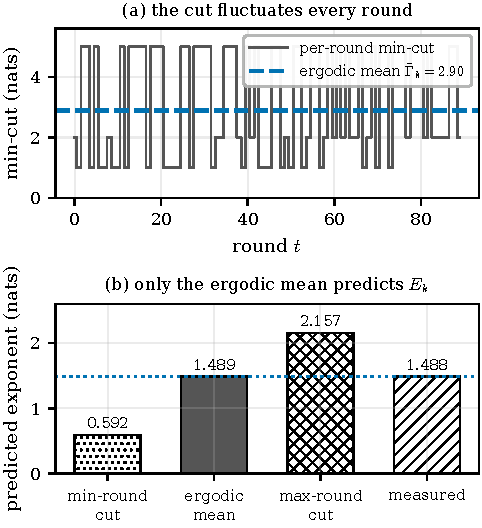
\includegraphics[width=\columnwidth]{fig_dynamic.pdf}
\caption{For a time-varying topology the binding rate is the ergodic mean of the per-round cuts. (a) The per-round
minimum cut fluctuates between one and five nats while its ergodic mean is $2.895$ nats. (b) Only the ergodic-mean
predictor matches the measured exponent, giving $1.489$ against $1.488$ nats, while the minimum-round and
maximum-round predictors are far off. The measured bar equals the ergodic-mean bar and not either extreme, which
is the content of Lemma~\ref{lem:aggregate}.}
\label{fig:dynamic}
\end{figure}

\subsection{The finite-length correction}
Because the exponent is approached from below, an engineer also needs the finite-length penalty, which the last
experiment checks. It validates the dispersion term that serves as the baseline for the
corrections used throughout. Fitting the exact errors to the second-order form confirms that the coefficient of
the square-root term scales linearly in the inverse Gaussian tail of the Type-I level with the square root of the
relative-entropy variance as its slope, and the analytic variance $V=1.5983$ is recovered as $1.6008$, an error
of two parts in a thousand. Table~\ref{tab:dispersion} lists the coefficients across five Type-I levels, whose fit
has a mean absolute error of $0.0013$. This confirms that the correction used elsewhere is the correct
theoretical term and that the exponent is approached at the predicted rate.

\begin{table}[t]
\centering
\caption{Second-order coefficients across Type-I levels for the base model, with $\tib=1.0202$ and $V=1.5983$. The
measured coefficient matches the predicted $\sqrt V\,\Phi^{-1}(\varepsilon)$ to a mean absolute error of $0.0013$.}
\label{tab:dispersion}
\renewcommand{\arraystretch}{1.15}
\begin{tabular}{@{}cccc@{}}
\toprule
$\varepsilon$ & $\Phi^{-1}(\varepsilon)$ & measured $b$ & $\sqrt V\,\Phi^{-1}(\varepsilon)$ \\
\midrule
0.01 & $-2.326$ & $-2.9436$ & $-2.9411$ \\
0.05 & $-1.645$ & $-2.0811$ & $-2.0795$ \\
0.10 & $-1.282$ & $-1.6214$ & $-1.6202$ \\
0.20 & $-0.842$ & $-1.0648$ & $-1.0640$ \\
0.35 & $-0.385$ & $-0.4874$ & $-0.4871$ \\
\bottomrule
\end{tabular}
\end{table}

%% ===========================================================================
\section{Discussion and Limitations}\label{sec:discussion}
%% ===========================================================================
The validated result is the test against independence with conditionally independent observations, which is the
setting in which the converse is tight and the achievability closes it, and it is the canonical case in which the
distributed rate-limited exponent is known exactly. We are explicit about scope. The general pair of hypotheses is
a different problem whose one-link exponent is itself unresolved, and for it the theorem provides only the $\tsha$
converse. If the observations are correlated across agents, the converse survives with the true joint divergence
in place of the sum, and only the clean single-letter evaluability of the bottleneck functional is lost. If the
connectivity is not ergodic, the cut may not converge and is replaced by an upper limit, and adversarial links
only tighten a converse. The exponents we measure are the exact optimal-detector errors rather than the output of
a particular finite-complexity protocol, so the achievability is verified at the information-theoretic optimum and,
separately, with an actual finite-field code that attains the cut. The distributed second-order dispersion, which
would combine the cut variance with a quantization term, remains open, and our dispersion experiment validates
only the centralized-cut baseline that forms its first component. These boundaries are consistent with the numbers
reported above and mark the natural directions for extension.

%% ===========================================================================
\section{Conclusion}\label{sec:conclusion}
%% ===========================================================================
We have determined the exact Type-II error exponent of fusion-free rate-constrained decentralized detection over
time-varying directed networks for a test against independence. The exponent is the smaller of the centralized
Stein value and the information-bottleneck relevance at the ergodic minimum cut, and a converse and a
type-preserving network-coding achievability meet at this value with no gap over graphs that may contain cycles
and may change with time. The cut is a sufficient statistic for the network, the binding rate for a changing graph
is the average of the per-round cuts, and network coding is necessary rather than convenient for the fusion-free
setting. A Gaussian instantiation turns the result into a water-filling rule for sharing a budget among unequal
agents, and an exact optimal-detector measurement, a genuinely routed network, and an actual finite-field code
confirm every prediction to within a few thousandths of a nat. The practical message is that designing such
systems for average throughput alone is not enough, because the decision quality at an agent is set by the
tightest cut that separates it from the evidence, aggregated over the changing topology. The natural next steps
are the distributed dispersion, an explicit symbol-level code, and the general-pair converse.

%% ===========================================================================
\bibliographystyle{IEEEtran}
\bibliography{../References/refs}

\end{document}
